%\subsection{Combinatorial Optimization and Computational Complexity}
%\label{sec:cop_and_cc}

Lawlers (1976) \cite{COP_book_lawler}, defined combinatorial analysis as "the mathematical study of the arrangement, grouping, ordering, or selection of discrete objects, usually finite in number". Schrijver (2002) \cite{COP_book}, following this definition of Lawlers, improves it with the important concept of optimal solution, "Combinatorial optimization searches for an optimum object in a finite collection of objects.". This definition is followed by a remark, stating that "typically, the collection (...) grows exponentially in the size of the representation", and concluding that "scanning all objects one by one and selecting the best is not an option".

Following a more concise definition \cite{aco_overview_advances}, a combinatorial optimization problem (COP) may be defined as follows:

\textbf{Definition 1)}  A combinatorial optimization model $P = (S,\Omega, f)$ consists of:
\begin{enumerate}
  \item a search space $S$, defined by a finite set of decision variables, each with a domain;
  \item a set $\Omega$ of constraints amongst the decision variables;
  \item an objective function $f$: $S$ $\rightarrow$ $\mathbb{R}_{0}^{+}$, to be minimized.
\end{enumerate}

The search space is defined by a set of decision variables $X_{i}, i = (1,...,n)$, each associated to a domain $D_{i}$, which specifies the possible value of each decision variable. An instantiation of a variable is an assignment of a value $v_{i}^{j} \in D_{i}$ to a variable $X_{i}$. This leads to the definition of a feasible solution $s \in S$, which corresponds to the assignment of a value to each decision variable, according to its domain, in such a way that all constraints in $\Omega$ are satisfied. Finally, the objective of the problem is to find a global minimum of P, that is, a solution $s^{*} \in S$ such that $f(s^{*}) \leq f(s)$ $\forall s \in S$. The set of all global minima is denoted by $S^{*} \subseteq S$.

When working on combinatorial optimization problems, it is useful to have an idea of how difficult the problem is. This characterization is provided by a field called computation complexity. A COP, $\Pi$, is said to have worst-case time complexity  $O(g(n))$, if the best algorithm 
for solving $\Pi$ finds an optimal solution to any instance of size $n$ of $\Pi$,
in a computation time upper bounded by $g(n)$.

A problem $\Pi$ is said to be solvable in polynomial time if the maximum amount of computing time that is necessary to solve any instance of size $n$ 
is bounded by a polynomial in $n$. If $k$ is the largest exponent of such a polynomial,
then the combinatorial optimization problem is said to be solvable in $\mathcal{O}(n^k)$ time.

Hence, a \textit{polynomial time algorithm} is characterized by a computation time bounded by $\mathcal{O}(p(n))$, for some polynomial function $p$, 
where $n$ is the size of the problem instance.  If 
an algorithm has a computational time that can not be bound by a polynomial function is denoted as an \textit{exponential time algorithm}.
Any problem that can be solved in polynomial time is said to be \textit{tractable}, while problems that 
are not solvable in polynomial time are called \textit{intractable}.

In the field of computational complexity, there is also another important concept called \textit{polynomial time reductions},
which transform a problem into another problem, in polynomial time. If the latter 
is solvable in polynomial time, than so is the first one. The class of problems which is solvable in polynomial time is called $P$.
On the other hand, there is a class of problems called $NP$, which stands for \textit{non-deterministic polynomial acceptable problems},
for which given a solution can be \textit{verified} in polynomial time.    
The class of NP-complete refers to the most difficult problems in NP.

It is worth mentioning that there exists another class, called NP-hard, for which each problem is as hard as the hardest NP-complete problem.
More precisely, a problem $H$ is NP-hard when every problem in NP can be reduced to $H$ using a polynomial time transformation.
This definition of the NP-hard class leads to the logical conclusion that finding a polynomial time algorithm for \textit{any} problem in NP-hard,
would imply the resolution of \textit{all} NP problems in polynomial time. However, until now, no polynomial time algorithm was found for any NP-hard problem.
Note that the class NP-hard does not necessary coincide with the class NP.

Regarding this, there is a discussion among the scientific community regarding the question "$P=NP?$",
since it is one of the major unsolved problems in computer science.
Figure \ref{fig:p_vs_np} illustrates this discussion by depicting the several classes, according to both possible solutions to the aforementioned question.
%src:: "https://en.wikipedia.org/wiki/NP-hardness#/media/File:P_np_np-complete_np-hard.svg
\begin{figure}[htpb]
  \centering
  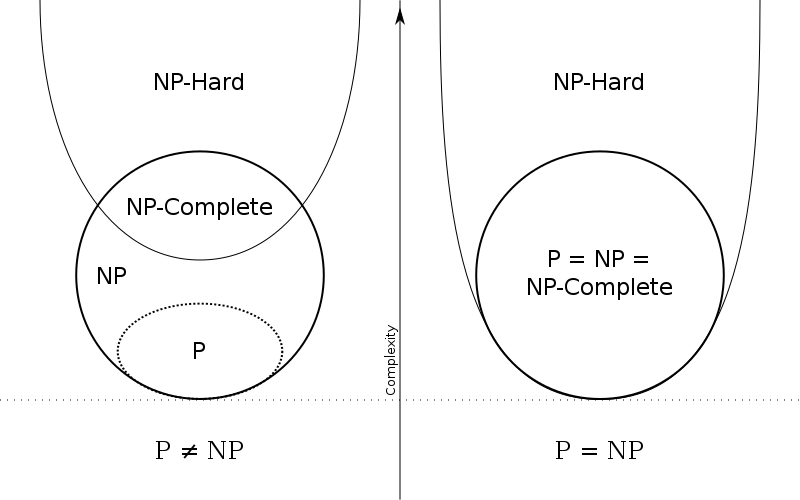
\includegraphics[width=.6\textwidth]{Figures/2.Chapter/p_vs_np.png}
	\caption{Illustration of the classes P, NP, NP-complete and NP-hard}
  \label{fig:p_vs_np}  
\end{figure}



